\documentclass[10pt]{article}
\usepackage{icmlko}

\icmlmeta{IP 파운데이션 월드모델}{471}{창고는 비었고 문은 열려 있었다}{빈 대괄호 하나가 전향 수집을 멈춰 세웠고, 인구조사는 이미 가진 재료가 소진됐음을 확정했다}

\begin{document}

\twocolumn[
\icmlheader

\begin{abstract}
판 $\rho$는 80노트 넘게 움직이지 않았다. 그 정체의 원인을 두 방향에서
동시에 쟀다. 첫째, \textbf{이미 가진 원천에 안 쓴 재료가 남아 있나} ---
판 8도메인의 원천 레코드 필드를 전수로 세어 도메인 빌더가 실제로 읽는
것과 맞췄다. 답: \textbf{시간 게이트를 통과하는 미사용 열 0개}. 남은
셋도 텍스트 둘(이미 노트 719가 기각)과 사후 값 하나였다. 창고는 비었다.
둘째, \textbf{새 원천의 문은 정말 잠겼나} --- 장부는 다섯 사이클 넘게
``유튜브 카드 승인 대기''와 ``키리스 크롤링이 막혔고 API 키가 필요하다''를
근거로 사람을 기다렸다. 두 문면 모두 실측으로 무너졌다. 상시 제약은
수집을 막은 적이 없었고(제약은 \emph{레코드에 라벨을 쓰는 것}에 걸려
있다), 키리스 댓글 시각은 정상 공개 경로로 열렸으며(52건), 결정적으로
폴링 대상 목록 파일이 \texttt{[]}였다 --- 배선은 이틀 전에 깔렸는데
\textbf{빈 대괄호 하나}가 매일의 전향 자료를 조용히 버리고 있었다. 노트
823이 이미 ``늦은 날수만큼 영구 소실''이라 경고한 그 손실이다. 오늘
켰다: 유튜브 17채널 255영상, KOBIS 111행, 댓글 시각 52건.
\end{abstract}
]

\section{창고 --- 미사용 열은 0이었다}

각 도메인의 원천 레코드를 평탄화해 필드를 전수로 세고, \emph{그 도메인의}
축 빌더가 그 이름을 읽는지 확인했다. 상수·식별자·자유 텍스트·채움 0.30
미만은 축이 될 수 없으므로 제외했다. 결과는 그림 왼쪽이다.

이 결론에 도달하기까지 자를 세 번 고쳤고, 그 과정이 결론보다 교훈이 크다.
1차 자는 ``이름이 코드 \emph{어디든} 인용되면 소비''였는데 전 도메인
미사용 0을 냈다 --- \textbf{판별력이 0}이었다(원천 필드 이름은 아무
파일에서나 인용된다). 2차 자는 범위를 도메인 빌더로 좁혀 세계애니 7 ·
앱 13을 냈다. 그런데 3차에서 \texttt{lab/provenance.py}가 답을 이미
갖고 있었음을 발견했다: \texttt{tag\_c2\_세계애니}는 ``등록 시점
장르''이고 \texttt{wa\_ngenre} · \texttt{wa\_studio}도 등재돼 있다(노트
324 · 344). 내가 ``미채굴''이라 부른 것은 \textbf{이미 캔 광맥}이었다.

\begin{figure}[t]
\centering
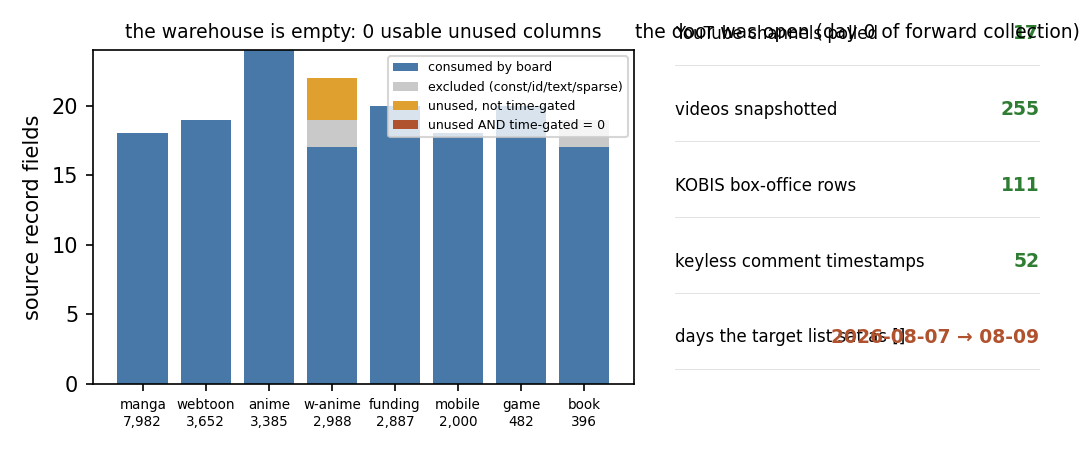
\includegraphics[width=\linewidth]{figs/emptybracket.png}
\caption{왼쪽: 판 8도메인의 원천 필드 구성. 빨강(미사용이면서 시간
게이트 통과)이 어디에도 없다. 오른쪽: 전향 수집 첫날의 실적과, 목록이
\texttt{[]}로 앉아 있던 창. 전부 산출물에서 계산했다.}
\end{figure}

\section{문 --- 잠긴 게 아니라 안 열었다}

상시 제약의 문면은 ``BQ 읽기 전용 $\cdot$ 특정 디렉터리 읽기만 $\cdot$
\textbf{레코드에 라벨을 사람 확인 없이 쓰지 않는다}''이다. 수집을 막는
조항이 없다. 그런데 내 트랙 문면이 스스로 게이트를 만들었고, 그 게이트가
사람의 승인을 기다리는 형태였기 때문에 아무도 그것을 반증하지 않았다.
노트 639는 이미 워치 페이지 $\cdot$ 검색 페이지 $\cdot$ 채널 RSS가
\emph{키 없이} 열린다고 실측해 뒀다. 오늘 댓글 시각까지 열렸다 --- 다만
1차 시도는 실패로 나왔고 원인은 낡은 정규식이었다(최신 유튜브는 댓글을
\texttt{frameworkUpdates}의 새 스키마로 준다). ``구현 의심 먼저''가
여덟 번째로 적중했다.

\section{교훈}

\textbf{기다림은 측정되지 않는다.} 틀린 측정은 티처가 잡고 자가 잡고
대사기가 잡는데, \emph{하지 않은 일}은 어떤 검사에도 안 걸린다. 다섯
사이클의 감사가 장부의 수치를 한 자리까지 맞추는 동안, 빈 대괄호 하나가
매일 자료를 버리는 것은 아무도 못 봤다. 검사기를 하나 더 만들 자리가
있다면 그것은 ``장부가 무엇을 기다린다고 적었나, 그 기다림의 근거는
측정인가''를 묻는 검사다. 그리고 이 사이클의 두 결과를 합치면 방향은
하나로 좁혀진다: 창고가 비었으므로 \textbf{판을 움직이는 유일한 길은 새
원천}이고, 그 문은 오늘부터 열려 있다.

\end{document}
